\section{Let's Start: Creating a Visualisation}
\label{tutorial_03}

\tick{\textbf{Goals:} The objective of this section is to create a visualisation for an Event-B model of a simple lift system.}

\subsection{Creating a new Visualisation Template}

The easiest way to create a new visualisation template is to duplicate the default template \texttt{b\_template} that is included in the \texttt{workspace} folder of your \bms~installation.
Just duplicate the \texttt{b\_template} folder and rename it to \texttt{lift}.
After refreshing your browser, the a new folder called \texttt{lift} should appear in your workspace (see Figure~\ref{fig_tut_01_workspace}).
Navigate to the \texttt{lift} folder. 
The folder contains three files:
\begin{itemize}
\item \texttt{template.html}: This file is the root file of your visualisation. It contains the actual visualisation and it's configuration.
\item \texttt{template.groovy}: The Groovy script file is the place where you can setup your observers.
In particular, the Groovy script file is the link between the formal model and the visualisation.
It allows you to programmatically control the ProB animator and to access the actual formal model being visualised.
In addition, you can register functions that can be called from the visualisation, e.g. executing an Event-B event after pressing a button in the visualisation.
\item \texttt{template.js}: The JavaScript file is needed to initialise your visualisation.
Moreover, it is the starting point to take advantage of the JavaScript language.
There exist are a lot of libraries for JavaScript that you can apply to create custom visualisations.
% if they have specific needs in a particular domain. 
For instance, it exists libraries for manipulating the DOM of an HTML document, or for generating chart and plot diagrams.
In addition, you can call functions that are registered in the Groovy script file.
This enables you to add some interactivity to your visualisation.
For instance, pressing a button in your visualisation could cause the execution of an Event-B event.
\end{itemize}

\begin{figure}[!ht]
\begin{center}
	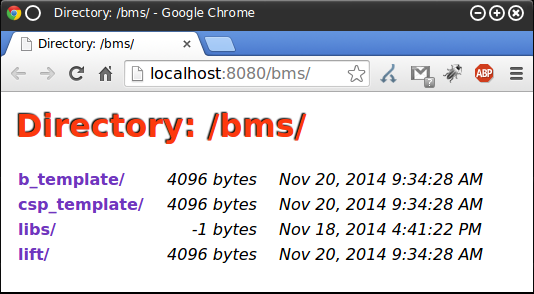
\includegraphics[width=12cm]{img/tutorial/tut_01.png}
	\caption{\bms~Workspace}
	\label{fig_tut_01_workspace}
\end{center}
\end{figure}

\subsection{The Formal Model}

We are going to create a visualisation for a simple lift system that allows movement of a single lift cage between three floors.
The door of the lift can be closed and opened - all in response to the pressing of floor call and cage send buttons.

You can download the Event-B model \file{EventBLift.zip}{here}.
Decompress it and put the files into a new folder called \texttt{model} relative to your \texttt{template.html} file in your workspace.

\subsection{Linking a Model with the Visualisation}

The next step consists of linking the model with the visualisation.
For this, open the \texttt{template.html} file with a text editor of your choice and add the following line within the head tag:

\begin{lstlisting}[language=html]
<meta name="bms.model" content="model/MLift.bcm" />
\end{lstlisting}

We link the visualisation with the Event-B machine called ``MLift''.
Linking a model within the \texttt{template.html} file automatically loads the model, when starting the visualisation.
Your \texttt{template.html} file should look like:

\begin{lstlisting}[language=html]
<html>
  <head>
      <title>BMotion Studio for ProB</title>
      <meta name="bms.model" content="model/MLift.bcm" />
      <meta name="bms.tool" content="BAnimation" />
      <meta name="bms.script" content="template.groovy" />
      <script data-main="template" src="/bms/libs/requirejs/require.js"></script>
  </head>
  <body>
  </body>
</html>
\end{lstlisting}

\info{The meta tag \textit{bms.script} (line 6) contains the link to the Groovy script file and the meta tag \textit{bms.tool} (line 5) defines the formalism or the simulator respectively that should be used. In this case we are creating a visualisation for a ``BAnimation'' (Classical-B or and Event-B).}

\subsection{Creating the Actual Visualisation}

The next step consists of creating the actual visualisation.
The user is not restricted to an editor in order to create a visualisation.
The user can make use of any tool that support the creation of SVG graphics or HTML documents.
%For this tutorial we are going to use the Inkspace\footnote{\url{https://inkscape.org}} editor. Inkscape is an editor for creating vector graphics that is available for Windows, Mac OS X and Linux.
%It's free and open source.
%With Inkscape the user can export the vector graphic into the SVG format.

%\info{We are currently working on a build-in graphical editor for creating SVG graphics and for managing observers.}

%\begin{figure}[!ht]
%\begin{center}
%	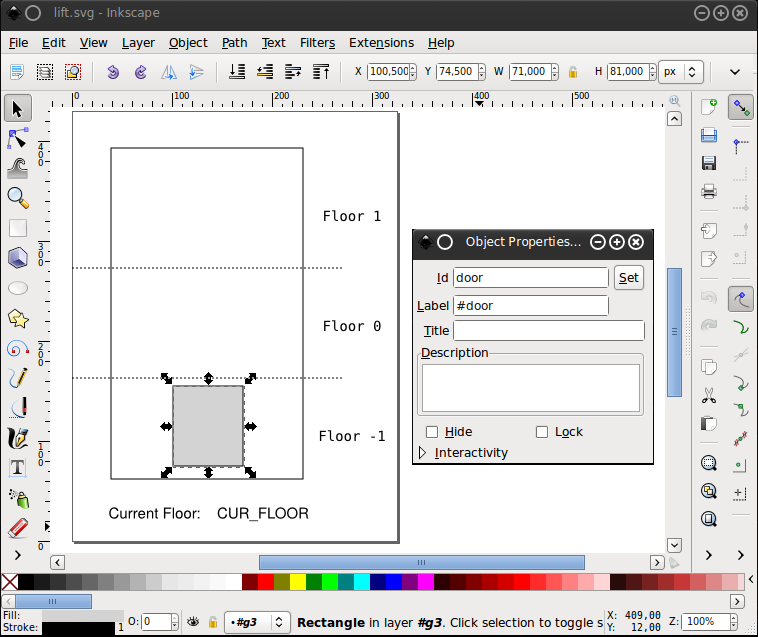
\includegraphics[width=12cm]{img/tutorial/tut_02.png}
%	\caption{Creating an SVG graphic with Inkscape}
%	\label{fig_tut_02_inkscape}
%\end{center}
%\end{figure}
Please download the prepared \file{lift.svg}{lift.svg} file and put it relative to your \texttt{template.html} file in your workspace.
Add the following tag within the body tag in your \texttt{template.html} file:

\begin{lstlisting}[language=html]
<object data="lift.svg" type="image/svg+xml" data-bms="svg">
</object>
\end{lstlisting}

%open it with Inkscape as demonstrated in Figure~\ref{fig_tut_02_inkscape}.
%Feel free to modify and explore the SVG graphic.
%In order to link visual elements of the SVG graphic with the formal model, we have to give them identifiers. 
%For this, select an element, open the context menu and select \textsf{Object Properties}.
%A popup window should be opened as demonstrated in Figure~\ref{fig_tut_02_inkscape}.
%As an example, we give the visual element that represents the door, the id ``door''.
%In Section~\ref{sec_creation_observers} we explain how we can use this information in order to create the link between the formal model and the visualisation by means of observers.
%If you are satisfied with your SVG graphic, save it as a plain SVG graphic with \textsf{File $\rangle$ Save As}.
%Select \textsf{Plan SVG (*.svg)} as an output format and click on the \textsf{Save} button.
%You can save the SVG file anywhere on your local system. 
%Open the SVG file with a text editor of your choice and put the SVG code within the body tag in the \texttt{template.html} file located in your workspace.
%Your \texttt{template.html} file should look like in Listing~\ref{lst:lifthtml}.

%\begin{lstlisting}[float=ht,language=html, ,caption={Template HTML file with Lift SVG graphic},label=lst:lifthtml]
%<html>
%  <head>
%      <title>BMotion Studio for ProB</title>
%      <meta name="bms.model" content="model/MLift.bcm" />
%      <meta name="bms.tool" content="BAnimation" />
%      <meta name="bms.script" content="template.groovy" />
%      <script data-main="template" src="/bms/libs/requirejs/require.js"></script>
%  </head>
%  <body>
%      <svg width="325" height="430" xmlns="http://www.w3.org/2000/svg">
%            <rect stroke="#000000" id="svg_1" height="331" width="192" y="37" x="39" fill="#ffffff" />
%            <line id="svg_2" y2="267" x2="270" y1="267" x1="0" stroke-dasharray="2,2" stroke="#000000" fill="none" />
%            <line id="svg_4" y2="157" x2="270" y1="157" x1="0" stroke-dasharray="2,2" stroke="#000000" fill="none" />
%            <rect fill="lightgray" stroke="#000000" x="101" y="275" width="70" height="80" id="door" />
%            <text font-weight="normal" xml:space="preserve" text-anchor="middle" font-family="Monospace" font-size="14" id="txt_floor1" y="110" x="280" stroke-dasharray="2,2" stroke-width="0" stroke="#000000" fill="#000000">Floor 1</text>
%            <text id="txt_floor0" font-weight="normal" xml:space="preserve" text-anchor="middle" font-family="Monospace" font-size="14" y="220" x="280" stroke-dasharray="2,2" stroke-width="0" stroke="#000000" fill="#000000">Floor 0</text>
%            <text id="txt_floor-1" font-weight="normal" xml:space="preserve" text-anchor="middle" font-family="Monospace" font-size="14" y="330" x="280" stroke-dasharray="2,2" stroke-width="0" stroke="#000000" fill="#000000">Floor -1</text>
%            <text fill="#000000" stroke="#000" stroke-width="0" x="145" y="407.5" id="txt_cur_floor" font-size="15" font-family="Helvetica, Arial, sans-serif" text-anchor="left" xml:space="preserve">CUR_FLOOR</text>
%            <text fill="#000000" stroke="#000" stroke-width="0" x="36.5" y="407.5" id="svg_3" font-size="15" font-family="Helvetica, Arial, sans-serif" text-anchor="left" xml:space="preserve">Current Floor:</text>
%    </svg>
%  </body>
%</html>
%\end{lstlisting}

\subsection{Starting the Visualisation}

Let's try out the visualisation!
In your browser, navigate to the \texttt{lift} folder and click on the \texttt{template.html} file.

The visualisation should start.
At the right bottom you will find a menu called \textsf{Open View} for opening different ProB related views.
For instance, Figure~\ref{fig_tut_03_running1} shows the running Lift visualisation with the ProB Events view opened.

At the moment nothing spectacular happens when changing the state (i.e. executing events in the Event view), because no link between visual elements and the formal model exists yet.
In the next Section we learn creating observers.

\begin{figure}[!ht]
\begin{center}
	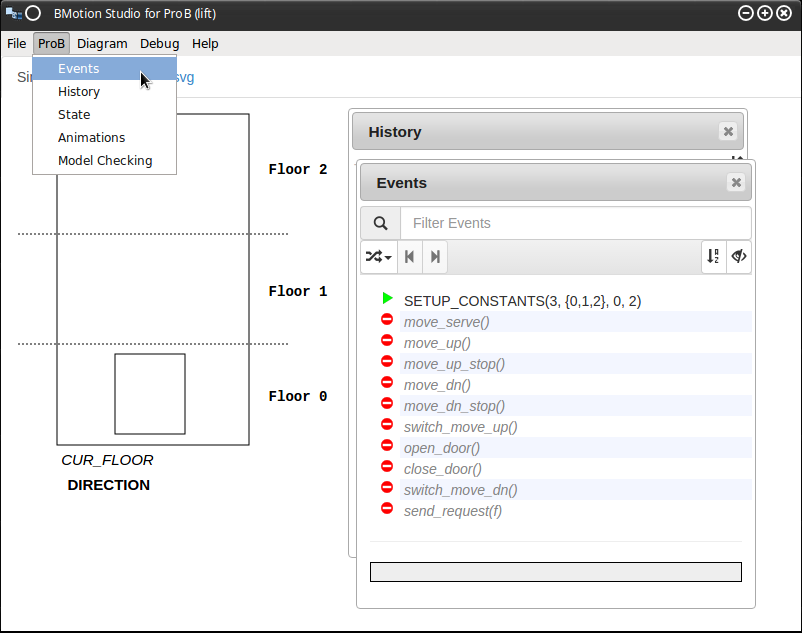
\includegraphics[width=12cm]{img/tutorial/tut_03.png}
	\caption{Running the Lift Visualisation for the First Time}
	\label{fig_tut_03_running1}
\end{center}
\end{figure}

\subsection{Creating Observers}
\label{sec_creation_observers}

Observers are used to link visual elements with the model. 
An observer is notified whenever a model has changed its state, i.e. whenever an event has been executed. 
In response, the observer will query the model's state and triggers actions on the linked visual elements in respect to the new state.
As an example, consider the following observer written in Groovy:

\begin{lstlisting}[float=ht,language=Groovy, caption={Transform Observer Displaying the Current Floor (Groovy)}]
transform("#txt_cur_floor") {
    set "text", { bms.eval("cur_floor").value }
    register(bms)
}
\end{lstlisting}

We are going to explore the Groovy code line by line.
Line 1 means that we want to transform the visual element with the id \textit{txt\_cur\_floor} that is located in our \texttt{template.html} file.
\bms~follows the jQuery selector syntax\footnote{\url{http://api.jquery.com/category/selectors}} to select elements.
The prefix ``\#'' denotes that we want to select an element by its id.
Line 2 affects that the attribute \textit{text} will be set to the value that is returned by the followed closure.
In particular, the closure evaluates the expression \textit{cur\_floor} in the current state and returns the value to be set.
In other words, the observer sets the current value of the variable \textit{cur\_floor} into the visual text element with the id \textit{txt\_cur\_floor}.
Line 3 is responsible to register the observer.
All registered observer will be triggered after every state change.

Let's create another observer.
Check out the following code:

\begin{lstlisting}[float=ht,language=Groovy, caption={Transform Observer for the Lift Door (Groovy)}]
transform("#door") {
    set "fill", { (bms.eval("door_open").value == "TRUE") ? "white" : "lightgray" }
    set "y", {
        switch (bms.eval("cur_floor").value) {
            case "-1": "275"
                break
            case "0": "175"
                break
            case "1": "60"
                break
            default: "275"
        }
    }
    register(bms)
}
\end{lstlisting}

Line 1 means that we want to transform the visual element with the id \textit{door}, similar to the previous observer.
Line 2 affects that the attribute \textit{fill} will be set to the value that is returned by the followed closure.
Whenever the expression \textit{door\_open} evaluates to \textit{TRUE}, the value \textit{white} (denoting the door is opened) is returned, otherwise the value \textit{lightgray} (denoting the door is closed) is returned.
Line 3 to 17 will switch the \textit{y} coordinate of the door (denoting the movement of the door between floors) according to the evaluation result of the expression \textit{cur\_floor}.
In line 18 we register the observer.
You can use the entire Groovy power and feature range for defining your observers.

Add both snippets to your \texttt{template.groovy} file and refresh your browser.
Let's see how this affects the visualisation:
Setup and initialise the machine using the ProB events view.
Execute some events and see what happens.
For instance, Figure~\ref{fig_tut_04_running2} shows the visualisation where the lift is on floor 0 and the door is open.

\begin{figure}[!ht]
\begin{center}
	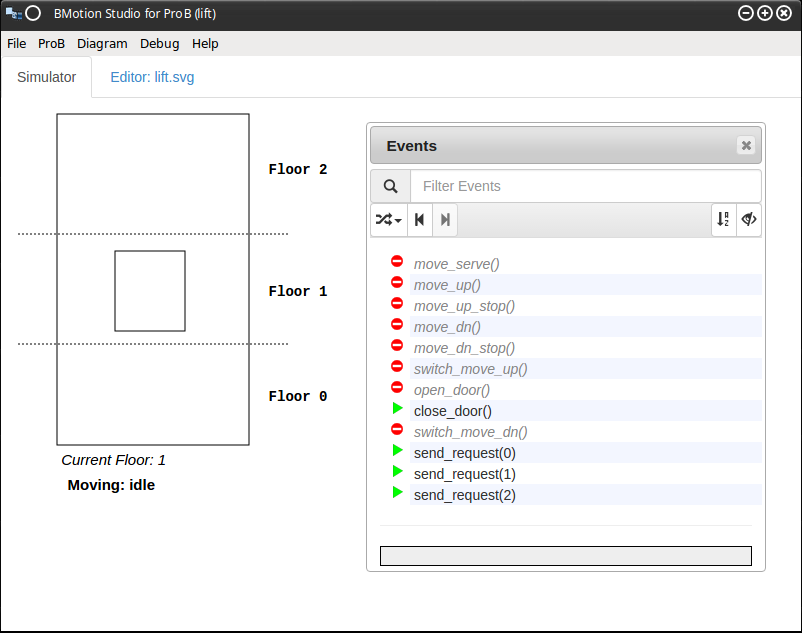
\includegraphics[width=12cm]{img/tutorial/tut_04.png}
	\caption{Lift Visualisation with Transformer Observer}
	\label{fig_tut_04_running2}
\end{center}
\end{figure}

\subsection{Add Interactivity}

In this Section we learn how we can enhance our visualisation with interactive features, like executing some Event-B events by clicking on some buttons.

Let's add an interactive feature, where the user can click on a floor label to order the lift on the corresponding floor.
Add the code snippet to your \texttt{template.js} file:
\newpage
\begin{lstlisting}[language=JavaScript, caption={Example of an Interactive Feature (JavaScript)}]
$("text[data-floor]").each(function () {
	$(this).executeEvent("push_call_button", {
		predicate: "b=" + $(this).attr("data-floor")
	});
});
\end{lstlisting}

Refresh your browser, to apply these changes and try to click on a floor label.
This should call the Event-B event \textit{push\_call\_button} with the corresponding predicate.
%For instance, clicking on the floor Label ``Floor 1'' should execute the Event-B event \textit{push\_call\_button(1)}.

Let's add another interactive feature, where the user can click on the visual element that represents the door to open or close the door respectively.
%The first step consists of registering a new Groovy function that executes the corresponding event \textit{open\_door} or \textit{close\_door}.
%Add the code snippet to your \texttt{template.groovy} file:
%\begin{lstlisting}[language=Groovy, caption={Registering a Groovy Function (Groovy)}]
%bms.registerMethod("openCloseDoor", {
%    def Trace t = bms.getTool().getTrace()
%    def Trace newTrace = executeEvent(t, "open_door", []) ?: executeEvent(t, "close_door", [])
%    if (newTrace != null) {
%        animations.traceChange(newTrace)
%        return [newState: newTrace.getCurrentState().id]
%    }
%})
%
%def Trace executeEvent(t,name,pred) {
%    try {
%        t.execute(name, pred)
%    } catch(IllegalArgumentException e) {
%        null
%    }
%}
%\end{lstlisting}
%In Line 1 we register a new Groovy function called \textit{openCloseDoor}.
%The next lines show an example how we can use the ProB Java API.
%In Line 2 we get the current trace of the animation.
%In Line 3, we first try to execute the \textit{open\_door} event by means of a helper method called \textit{executeEvent} (Line 10 to 16).
%If the return value of the helper method is null (the event could not be executed), we try to execute the event \textit{close\_door}.
%If we success (we executed one of the both events), we trigger a trace change, causing to refresh the current animation (Line 5).
%This in turn changes the state and triggers our registered observers.
%Line 6 returns a Json object that contains the state id of the new state.
%This information can used later at the JavaScript side after executing the registered \textit{openCloseDoor} method.
%Let's switch to the JavaScript side.
Add the following code snippet to your \texttt{template.js} file:
%\begin{lstlisting}[language=JavaScript, caption={Call openCloseDoor Groovy Method (JavaScript)}]
%$("#door").click(function () {
%	bms.callMethod("openCloseDoor", {
%		callback: function (data) {
%			console.log("Callback: " + data)
%		}
%	})
%}).css("cursor", "pointer")
%\end{lstlisting}
\begin{lstlisting}[language=JavaScript, caption={Interaction with the Lift Door (JavaScript)}]
$("#door").executeEvent("open_door", {
	alternative: [ {name: "close_door"} ],
	callback: function (data) {
		console.log("Callback: " + data)
	}
});
\end{lstlisting}

In Line 1 we register a new execute event handler on the visual element with the id door.
The execute event handler executes the event \textit{open\_door}, whenever it is enabled in the current state.
In line 2 we register one alternative event \textit{close\_door}.
The alternative event is executed, whenever the registered event \textit{open\_door} is disabled.
%Line 2 calls our registered Groovy method \textit{openCloseDoor}.
In Line 3 to 5 we pass a callback function that is called after an event (\textit{open\_door} or \textit{close\_door}) was executed.
%In this case we print the returned new state id on the console.

These are only small examples for adding interactivity to your visualisation.
In particular you are not limited to these examples.
You can download the final visualisation \file{LiftVisualisation.zip}{here}.

